\documentclass{report}
\usepackage[a4paper, margin=0.5in]{geometry}
\usepackage{parskip}
\usepackage{graphicx}
\usepackage{caption}
\usepackage{amssymb}
\usepackage{amsmath}
\usepackage{algpseudocode}
\usepackage{algorithm}

\captionsetup[figure]{
  font = it,
  labelfont = bf
}

\begin{document}
\begin{minipage}[b]{0.48\textwidth}
  \section*{Hamerly's Algorithm}
  Hamerly's algorithm is an optimization of the standard algorithm and expoits the fact that it is not necessary to recalculate the distance of each point from the centroids each time the latter are repositioned. Using the triangular inequality it is, in fact, possible to identify critical points, that is, points for which it is necessary to recalculate the distance to each centroid to find the closest one. In contrast, for the other points, the class to which they were assigned remains the right one even if the centroid has been moved.

  \section*{Triangular inequality}
  Given 3 points A, B, C $\in \mathbb{R}^2$ then  
  \begin{equation}
    |d(A, C) - d(B, C)| \leq d(A, B) \leq d(A, C) + d(B, C)
  \end{equation}
  \begin{equation}
    |d(A, B) - d(C, B)| \leq d(A, C) \leq d(A, B) + d(C, B)
  \end{equation}
  \begin{equation}
    |d(C, A) - d(B, A)| \leq d(C, B) \leq d(C, A) + d(B, A)
  \end{equation}
  Where $d(\alpha, \beta)$ is the euclidian distance between the points $\alpha$ and $\beta$. This inequality can also be interpreted geometrically: referring to Figure \ref{fig:triineq}, any side of a triangle is lower than (or equal) to the sum of the other two sides and it is higher (or equal) than the absolute value of the difference between the other two sides.

  \hspace{0.1in}
  \begin{center}
    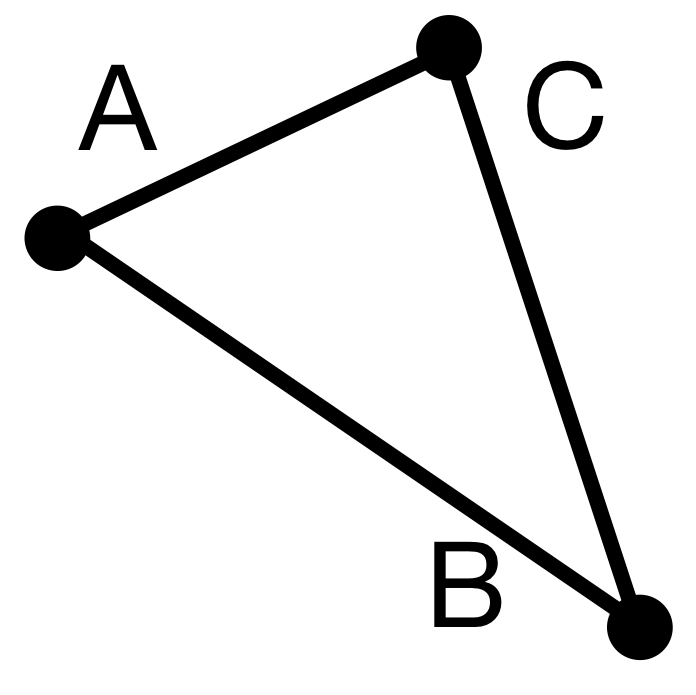
\includegraphics[width = 0.25\textwidth]{imgs/triangle.png}
    \captionof{figure}{3 points in space forming a triangle}
    \label{fig:triineq}
  \end{center}

  \subsubsection*{Triangular inequality and k-means}
  For simplicity, let us assume that we have only one point and two centroids (Figure \ref{fig:triCC}).  

  \begin{center}
      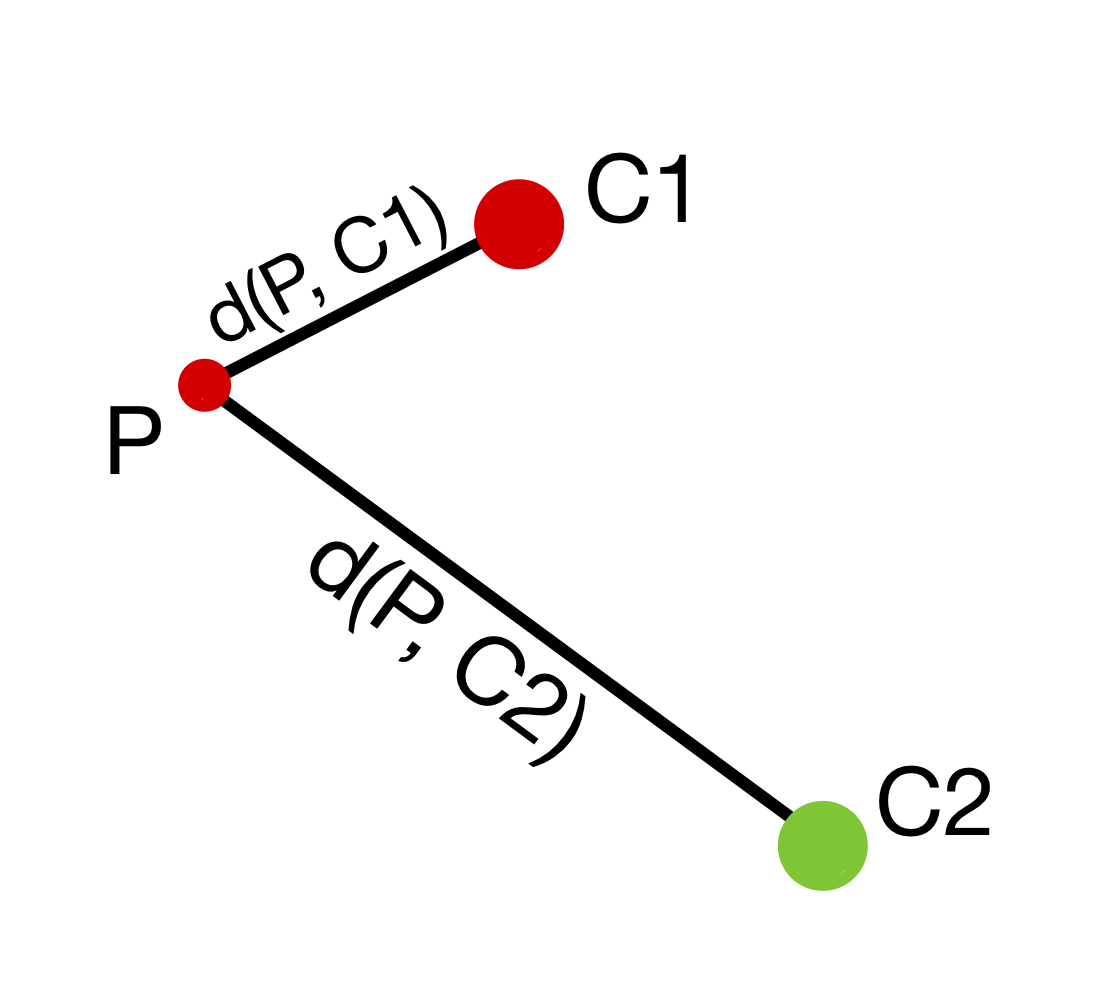
\includegraphics[width = 0.3\textwidth]{imgs/triCC.png}
      \captionof{figure}{Example with 2 centroids and one point}
      \label{fig:triCC}
  \end{center}

  At this point we assume that the centroids shift (Figure \ref{fig:triCCafter}), because of the other points (which are not represented).

  \begin{center}
      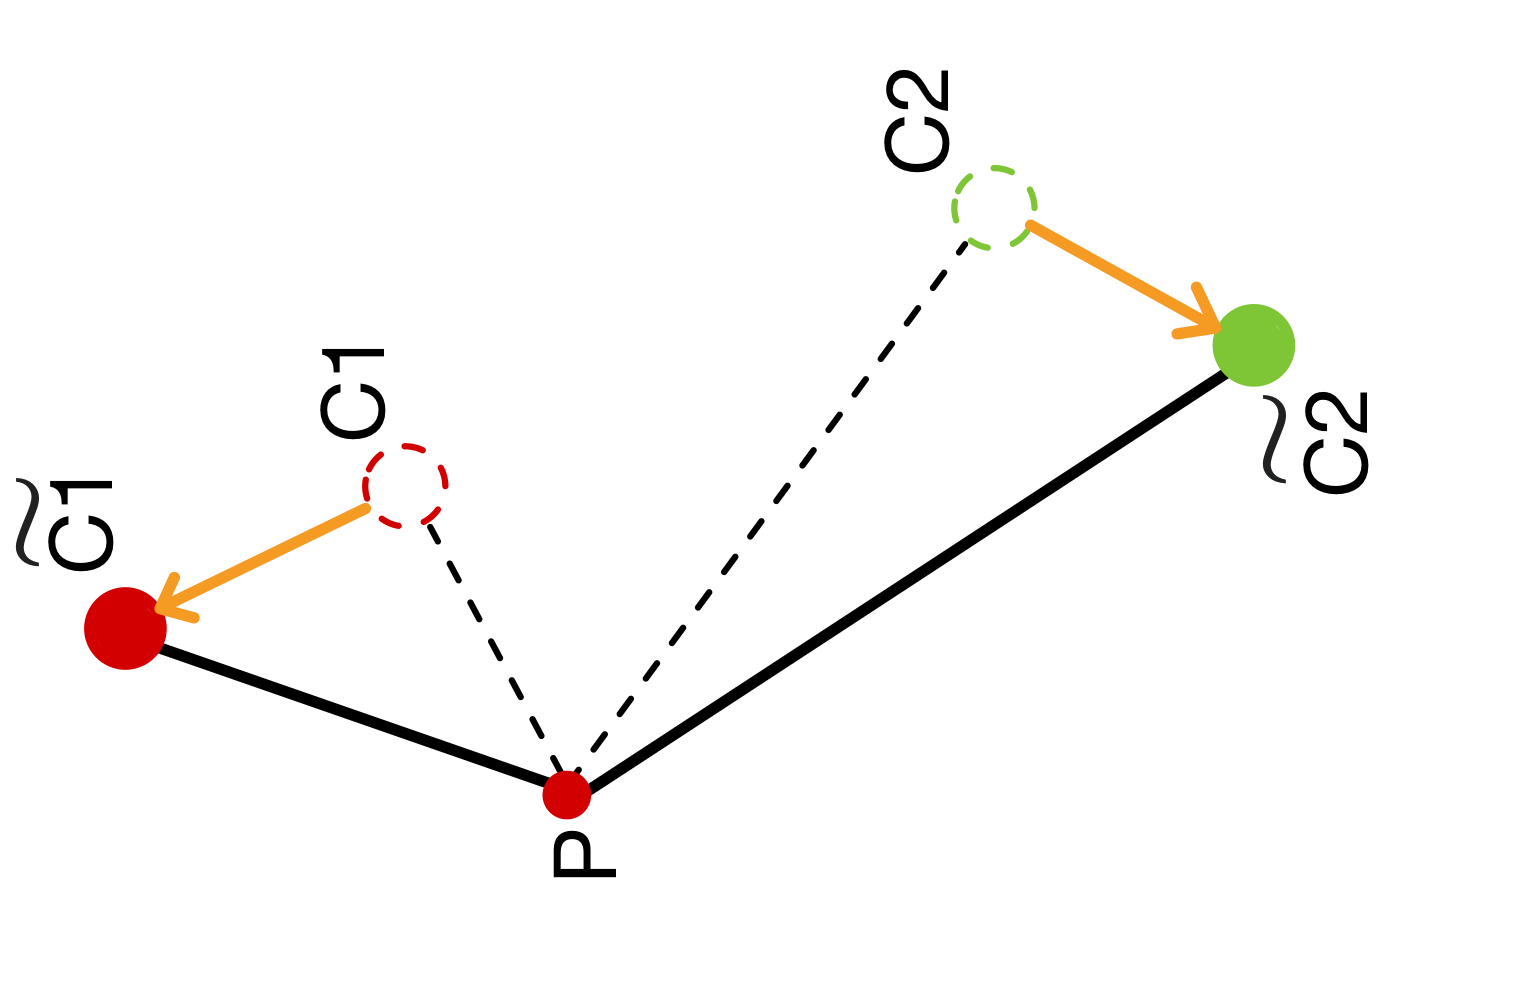
\includegraphics[width = 0.6\textwidth]{imgs/triCCAfter.png}
      \captionof{figure}{Example after the centroids have shifted}
      \label{fig:triCCafter}
  \end{center}   
\end{minipage}
\hspace{0.1in}
\begin{minipage}[b]{0.48\textwidth}
  Thanks to the triangular inequality, we can state that the distance between P and $\tilde{C_1}$ is:
  \begin{equation*}
    |d(P, C_1) - d(C_1, \tilde{C_1})| \leq d(P, \tilde{C_1}) \leq d(P, C_1) + d(C_1, \tilde{C_1})
  \end{equation*}
  And in the same way:
  \begin{equation*}
    |d(P, C_2) - d(C_2, \tilde{C_2})| \leq d(P, \tilde{C_2}) \leq d(P, C_2) + d(C_2, \tilde{C_2})
  \end{equation*}

  Using this result, we can improve the k-means algorithm as follows.
  The first step remains mostly unchanged: it consists of assigning to each point the nearest centroid, and to do this it is necessary to calculate all the distances between the point and the centroids. The difference with the standard algorithm is that in this case, for each point, we will save the distance to the nearest centroid, called upper bound (ub), and also the distance to the second nearest centroid, called lower bound (lb).

  For example, if for a point (P) the nearest centroid is $C_1$ we have that
  \begin{equation}
      ub = d(P, C_1)
  \end{equation}
  \begin{equation}
      lb = \min\limits_{j \neq 1} d(P, C_j)
  \end{equation}

  After the first step, the centroids are repositioned and again the algorithm is almost identical: eqs \ref{eq:centrep} is used to compute the new position of the centroids, but unlike before we will also save the distance traveled by each centroid (using an array with length K called cdistaces), the distance traveled by the centroid that moved the most (maxdist) and its index (maxdist\_index) and the distance traveled by the second centroid that moved the most (secmaxdist).

  At this point, the parameters $ub$ and $lb$ are updated for each point p, as follows.

  \begin{equation}
    ub =  ub + cdistances[p.centroid\_index]
  \end{equation}
  If the closest centroid is also the one that moved the most then
  \begin{equation}
      lb = lb - secmaxdist
  \end{equation}
  Else
  \begin{equation}
      lb = lb - maxdist
  \end{equation}

  These updates are justified by the triangular inequation. In fact, we know that after that the centroids have moved, the point cannot be farther than $ub$ from the nearest centroid and at the same time cannot be closer than $lb$ from the second nearest one.

  Thanks to the previous step, it is possible to identify as critical the points for which $ub \geq lb$, that is, the points for which the assigned centroid may not be the nearest.
  
  The next step is to iterate for all points but recalculating the distance to the nearest centroid only for the critical ones. Moreover, we can optimize this process even more since, once a critical point has been found, it may be sufficient to recalculate only the upper bound, i.e., the distance to the nearest centroid, and then check again the condition $ub \geq lb$ and only if the condition is still verified then it will be necessary to carry out the full calculation of the distances.
  
  Finally, the centroids are updated and the procedure is repeated until the condition of convergence is reached or after a certain number of iterations.
\end{minipage}

\newpage

\begin{minipage}[b]{0.48\textwidth}
  \section*{Number of iterations}
  In the case of Hamerly's algorithm, the number of iterations required to complete the classification is:
  \begin{equation}
      d\cdot K\cdot N + md(\phi N\cdot K + (1 - \phi)N)
  \end{equation}
  Where $\phi$ is the percentage of critical points with respect to the total number of points.

  The improvement over the standard algorithm lies in the fact that only the first time it is necessary to compute all the distances, whereas in subsequent iterations, for most points, there is no need to recompute the nearest centroid.

  \section*{Parallelize the Hamerly's algorithm}
  The Hamerly's algorithm has three main sub-tasks: assignation of the points to a class, update of the centroids, update of the lower and upper bounds of all points.

  \subsubsection*{Assignation of the points to a class}
  In this phase, each point will be assigned to a centroid which will represent its class. If it is the first iteration, this can be easly parallelizable by simply partitioning the points between the threads. Each thread will then goes through its set of points and find the minimum distance between the point and the centroids and therefore will assign to point to that class. In this first ieration the work load is equally balanced across the threads because the work that has to be done for each point is the same.

  This is not true from the second iteration, because in this case the only points for which the minimum distance is calculated are the critical points. Therefore it is not enough to partion the points between the threads because criticals points could be not equally distribuited across the point set and because of this some threads could have more work to do compared to others. A load balancing tequiniche has to be used.

  \subsubsection*{Update of the centroids}
  This is the phase where the centroids are moved. Also this step can be easly parallized by simply partitioning the centroids between the threads which, for every of its centroid will compute the new position using the values inside the matrix average\_per\_class and points\_per\_class.

  The work load for every centroid is the same, therefore no special cautions are needed when parallelizing it.

  \subsubsection*{Update the lower and upper bounds of all points}
  During this step, the lower and upper bound of each points are updated using the information saved during the "Update of the centroids" (cdistances, maxdist, maxdist\_index and secmaxdist). This is where the balancing algorithm is applied and the result of this phase is an array (called criticals) containing the address of all critical points that have been found. 

  \subsubsection*{Reduction on the variables average\_per\_class and points\_per\_class}
  When parallelizing the code, a particular cautions has to be taken if two threads wants to add (or subtract) on the same variable.
\end{minipage}
\hspace{0.1in}
\raisebox{0in}{
\begin{minipage}[b]{0.48\textwidth}
  This is, in fact, the case for the matrix average\_per\_class and the array points\_per\_class. This is because when calculating the closest class, two threads could find two points that belong to the same class and therefore they both need to update the matrix and increment the array.

  To explain why this is a problem suppose we have a variable v = 42 and two threads that want to modify it as described by the following pseudocode

  \begin{algorithm}[H]
    \caption{Parallel update of a variable}
    \begin{algorithmic}
      \If {$thread\_id == 0$}
        \State v = v + 1
      \ElsIf{$thread\_id == 1$}
        \State v = v + 2
      \EndIf
    \end{algorithmic}
  \end{algorithm}

  The expected result is 45 (42 + 1 + 2), however if the code is executed the result might not be 45. This happens if the threads read at the same time the value of v (which is likely to happen in a parallel execution), in that case, they both read 42 and they modify it and then save it back in memory. What happens is that if thread zero is the last to save the value, v would be 43 and, in the same way, if thread one finish later v would be 44.

  The way to solve this problem is called reduction (in this case on the variable v): both thread will have a local memory where they make the changes and when they finish to execute, a sequential algorithm is executed that puts toghether all the changes that have been done.

  OpenMP offer a special clause for that: \#pragma omp parallel reduction(+:v). The first part "\#pragma omp parallel" is just the classic one to start a parallel section, while "reduction(+:v)" is the part that enable reduction. In particular the plus sign specify the operation that will be done by the sequential algorithm on the variable which is specified after the semicolumn. \\
  
  OpenMP also allows to reduce arrays, considering for example the points\_per\_class array, the clause would be: \#pragma omp parallel reduction(+:points\_per\_class[:K]). The same thing is not true for matrices: OpenMP doesn't support matrix reduction. But, it is possible to solve this problem by converting the matrix to an array.

  Let's consider the average\_per\_class $Kxd$ matrix, we can equivalently use an array with a length of $K\cdot d$. In this way we still have the same number of slots for the data and we can access the (i, j) element as by accessing the $(i \cdot d + j)$-th index

  \subsubsection*{Pattern for a parallel access}
  In this section, a general algorithm which has been used a lot in this implementation will be explained: how to partition a set of points between an arbitrary number of threads.

  Suppose that we have N points and T threads, if N was a multiple of T then it would be easy to split the data by using the following algorithm.
\end{minipage}}

\newpage

\begin{minipage}[b]{0.48\textwidth}
  \begin{algorithm}[H]
    \caption{Data partitioning if N mod T = 0}
    \begin{algorithmic}
      \State points\_per\_thread = N / T
      \State ------- Parallel Section -------
      \For{i $<$ points\_per\_thread}
        \State p = points[ points\_per\_thread $\cdot$ thread\_id + i ]
      \EndFor
      \State ----- End Parallel Section -----
    \end{algorithmic}
  \end{algorithm}

  The problem is that N and T are not known a priori and N could not be a multiple of T, therefore we need to properly handle those extra points. First we calculate the points per class and the remainder as
  \begin{equation}
    points\_per\_class = Int(\frac{N}{T})
  \end{equation}
  \begin{equation}
    remainder = N mod\hspace{0.05in} T
  \end{equation}

  Where Int(a) is the integer part of a.
  Thanks to the mod operator properties we know that $remainder < T$. At this point we can assign to the first threads an extra point which can be easly done by checking the thread id as follows:

  \begin{algorithm}[H]
    \caption{Add an extra points to the first threads}
    \begin{algorithmic}
      \State points\_per\_thread = Int(N / T)
      \State remainder = N \% T
      \State ------- Parallel Section -------
      \If {thread\_id $<$ remainder}
        \State points\_per\_class += 1
      \EndIf
      \State ...
      \State ----- End Parallel Section -----
    \end{algorithmic}
  \end{algorithm}

  Also the access pattern needs to be modified because not all threads have the same number of points assigned to them. \\

  The first threads access one more point than the others, therefore they overall introduce a shift equal to the remainder to the points that will be accessed from the last threads. The offset need , therefore, to be added only to the threads accessing a number of points equal to points\_per\_thread (and not points\_per\_thread + 1). The pseudocode then becomes:

  \begin{algorithm}[H]
    \caption{Add an extra points to the first threads}
    \begin{algorithmic}
      \State points\_per\_thread = Int(N / T)
      \State remainder = N \% T
      \State offset = remainder
      \State ------- Parallel Section -------
      \If {thread\_id $<$ remainder}
        \State points\_per\_thread += 1
        \State offset = 0
      \EndIf

      \For {i $<$ points\_per\_thread}
        \State p = points[points\_per\_thread $\cdot$ thread\_id + i + offset]
      \EndFor
      \State ----- End Parallel Section -----
    \end{algorithmic}
  \end{algorithm}

\end{minipage}
\hspace{0.1in}
\begin{minipage}[b]{0.48\textwidth}
  
\end{minipage}

\end{document}